% Quantum autoencoder of notebook 45, drawn for N = 6 and k = 2 (the code studies k = 1..4; trash = LAST k qubits).
% encode = hardware-efficient ansatz U(theta) on the input |psi>; trash qubits measured in Z and reset to |0>
% (equivalently: traced out and replaced by fresh |0>); decode = U^dagger(theta).
% Training cost: F_trash = probability that all trash qubits give 0.  Figure of merit: F_rec = <psi|rho_out|psi>.
\documentclass[tikz,border=4pt]{standalone}
\usepackage{amsmath,amssymb,bm}
\usetikzlibrary{arrows.meta,decorations.pathreplacing,calc}
\newcommand{\ket}[1]{\lvert #1\rangle}
\begin{document}
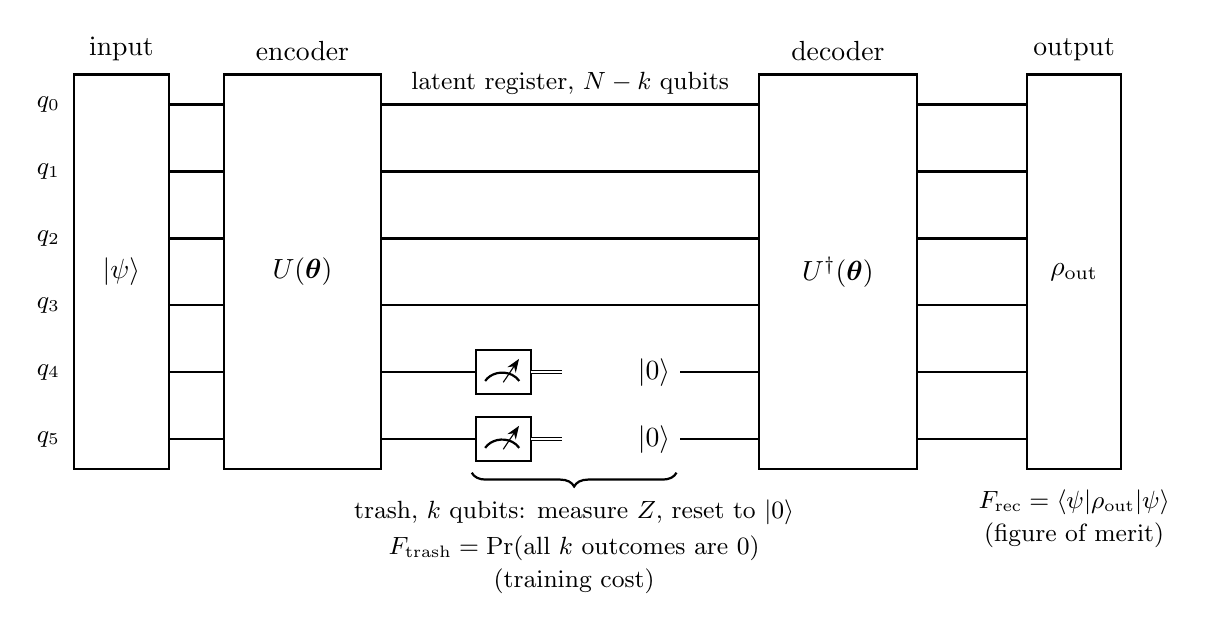
\begin{tikzpicture}[thick, >=Stealth, x=1cm, y=0.85cm]
  % input state
  \draw[fill=white] (-1.5,0.45) rectangle (-0.3,-5.45);
  \node at (-0.9,-2.5) {$\ket{\psi}$};
  \node[above] at (-0.9,0.5) {input};
  % wires: latent 0..3 run straight through, trash 4,5 are interrupted
  \foreach \y in {0,-1,-2,-3} \draw (-0.3,\y) -- (10.6,\y);
  \foreach \y in {-4,-5} { \draw (-0.3,\y) -- (3.6,\y); \draw (6.2,\y) -- (10.6,\y); }
  % qubit labels
  \foreach \q in {0,...,5} \node[anchor=east, font=\small] at (-1.55,-\q) {$q_{\q}$};
  % encoder
  \draw[fill=white] (0.4,0.45) rectangle (2.4,-5.45);
  \node at (1.4,-2.5) {$U(\boldsymbol\theta)$};
  \node[above] at (1.4,0.5) {encoder};
  % decoder
  \draw[fill=white] (7.2,0.45) rectangle (9.2,-5.45);
  \node at (8.2,-2.5) {$U^\dagger(\boldsymbol\theta)$};
  \node[above] at (8.2,0.5) {decoder};
  % latent register label
  \node[font=\small, above] at (4.8,0.0) {latent register, $N-k$ qubits};
  % trash: measure in Z, then a fresh |0>
  \foreach \y in {-4,-5} {
    \draw[fill=white] (3.6,\y+0.33) rectangle (4.3,\y-0.33);
    \draw (3.72,\y-0.13) arc (150:30:0.25);
    \draw[->, thin] (3.95,\y-0.15) -- (4.15,\y+0.2);
    \draw[double, thin] (4.3,\y) -- (4.7,\y);
    \node[anchor=east] at (6.2,\y) {$\ket{0}$};
  }
  \draw[decorate, decoration={brace, amplitude=5pt, mirror}] (3.55,-5.5) -- (6.15,-5.5)
       node[midway, below=6pt, font=\small, align=center]
       {trash, $k$ qubits: measure $Z$, reset to $\ket{0}$\\[2pt]
        $F_{\rm trash}=\Pr(\text{all $k$ outcomes are }0)$\\[1pt] (training cost)};
  \draw[fill=white] (10.6,0.45) rectangle (11.8,-5.45);
  \node at (11.2,-2.5) {$\rho_{\rm out}$};
  \node[above] at (11.2,0.5) {output};
  \node[font=\small, anchor=north, align=center] at (11.2,-5.6) {$F_{\rm rec}=\langle\psi\vert\rho_{\rm out}\vert\psi\rangle$\\[1pt] (figure of merit)};
\end{tikzpicture}
\end{document}
